\documentclass{article}
\usepackage[a4paper, total={6in, 9in}]{geometry}
\usepackage{fancyhdr}
\usepackage{amsmath}
\usepackage{algorithm}
\usepackage{algpseudocode}
\usepackage{CJK}
\usepackage{graphicx}

\newtheorem{theorem}{Theorem}
\newtheorem{lemma}{Lemma}
\newtheorem{proof}{Proof}[section]

\pagestyle{fancy}
\fancyhf{}
\rhead{1600017857}
\lhead{Homework(1)}
\rfoot{}
\cfoot{Page \thepage}

\title{Homework(1)}
\date{2018-03-01}
\author{
  \begin{CJK}{UTF8}{gbsn}
    黄道吉-1600017857
  \end{CJK}
}

\begin{document}
\begin{CJK}{UTF8}{gbsn}

\section{找到至少一个错误的图片,并给出正确图片,说明理由}
  \paragraph{}
    第13页的第二张图片是有误的,图为阿基米德,而希罗的图片应为这一张
    \begin{figure}[ht]
      \centering
      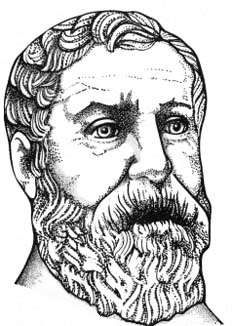
\includegraphics[scale=0.4]{Hero_of_Alexandria.png}
      \caption{图片来自Wikipedia}
      \label{fig:label}
    \end{figure}
  \paragraph{}
    其他的图片应该都是正确的,除了我没能找到Karush的照片,谷歌识图也没有结果

\section{举出更多"没有免费午餐"理论能应用的例子}
  \paragraph{}
    \textit{例1} 比方说要走短程的路程的话自行车比飞机方便,但是这并不说明在任何情况下自行车都比飞机方便,比方说从一个大洲飞到另一个大洲
  \paragraph{}
    \textit{例2} 不同的刀具适用的场景不同,指甲刀适合剪指甲和丝线之类的,菜刀适合切菜,等等,没有一种普世的刀具
\end{CJK}
\end{document}
